\documentclass[VM.tex]{subfiles}
\tikzset{
  load/.style   = {ultra thick,-latex},
  stress/.style = {-latex},
  dim/.style    = {latex-latex},
  axis/.style   = {-latex,black!55},
}

% Drawing View
\tikzset{dimetric2/.style={
  x={(0.935cm,-0.28cm)},
  y={(0.44cm, 0.312cm)},
  z={(0.000cm, 0.943cm)},
}}
\begin{document}

\subsubsection*{Description : }
It is the continuation of previous problem but the error of the solution is compared for different thicknesses. 


\subsubsection*{Material and Geometric data : }



\begin{table}[ht]
\renewcommand{\arraystretch}{1.5}
\centering
\caption{Input Data}

\begin{tabular}{|ll|ll|ll|}
\hline
\multicolumn{2}{|l|}{\cellcolor[HTML]{C0C0C0}Material Property} & \multicolumn{2}{l|}{\cellcolor[HTML]{C0C0C0}Geometric Data} & \multicolumn{2}{l|}{\cellcolor[HTML]{C0C0C0}Loading Data} \\ \hline  \hline
Young's Modulus ($E$)          & 1E11 $pa$         & Length ($a$)        & 1 $m$        & $N_2$    &  $\frac{T}{t}$ $N/m^2$      \\
Poission's Ratio ($\nu$)       & 0.3         & Breath ($b$)        & 40 $m$          &  Tension $T$      &    3E4 $N/m$    \\ 
Density ($\rho$)       & 7810 $Kg/m^3$         & Thickness($t$)        & \{0.001,0.005,..,0.5,1\} $m$          &    &        \\ \hline
\end{tabular}
\end{table}




\subsubsection*{Mesh and boundary condition : }


\begin{table}[h!]
\renewcommand{\arraystretch}{1.5}
\centering
\caption{FEM and Boundary condition data}
\label{my-label}
\begin{tabular}{|l|lll|l|l|}
\hline
 \multicolumn{4}{l|}{\cellcolor[HTML]{C0C0C0}Direchlet Boundary} & \multicolumn{2}{l|}{\cellcolor[HTML]{C0C0C0}Loading Conditions} \\ \hline \hline
Geo - \newline Entity      & $w$          & $\theta _ x$     & $\theta _ y $    & Geo - \newline Entity         & $N_2$         \\    \hline
                 line \{1,3\}                   & Fixed      & Free         & Free        & line \{1,3\}                   & $\frac{T}{t}$ $N/m^2$        

 \\ \hline
\end{tabular}
\end{table}

\subsubsection*{Result and error analysis : }
\begin{figure}[h!]
\centering
\resizebox{0.8\textwidth}{!}{
\begin{tikzpicture}
\begin{semilogxaxis}[xlabel=Thickness$(m)$,ylabel=error $\%$,xmin=0.001,xmax=1,ymin=-3,ymax=25
]
\addplot[
color=blue,
mark=square,
]
coordinates{(0.001,22.795)(0.005,3.394)(0.01,0.281)(0.05,0.018)(0.1,0.4)(0.5,3.119)(1,3.207)};

\end{semilogxaxis}
\end{tikzpicture}
}
\end{figure}





\begin{figure}[h!]
\centering
\begin{subfigure}{.8\textwidth}
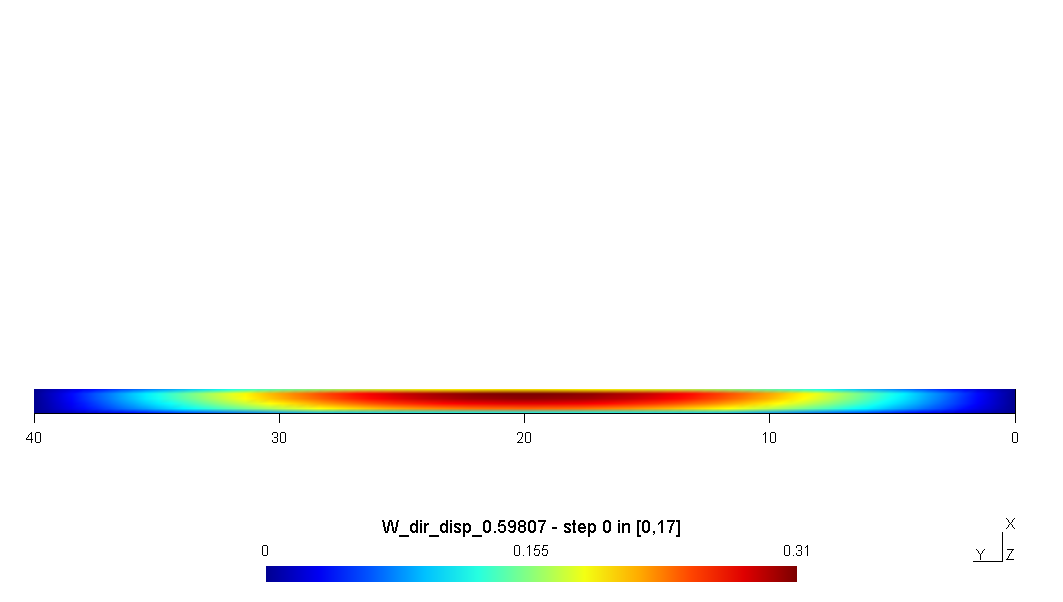
\includegraphics[width=\linewidth,trim={0 3cm 0 9cm},clip]{NAS277/t0_001.png}
\caption{Mode Shape 1 for thickness = 0.001 $(m)$}
\end{subfigure} \vfill
\begin{subfigure}{.8\textwidth}
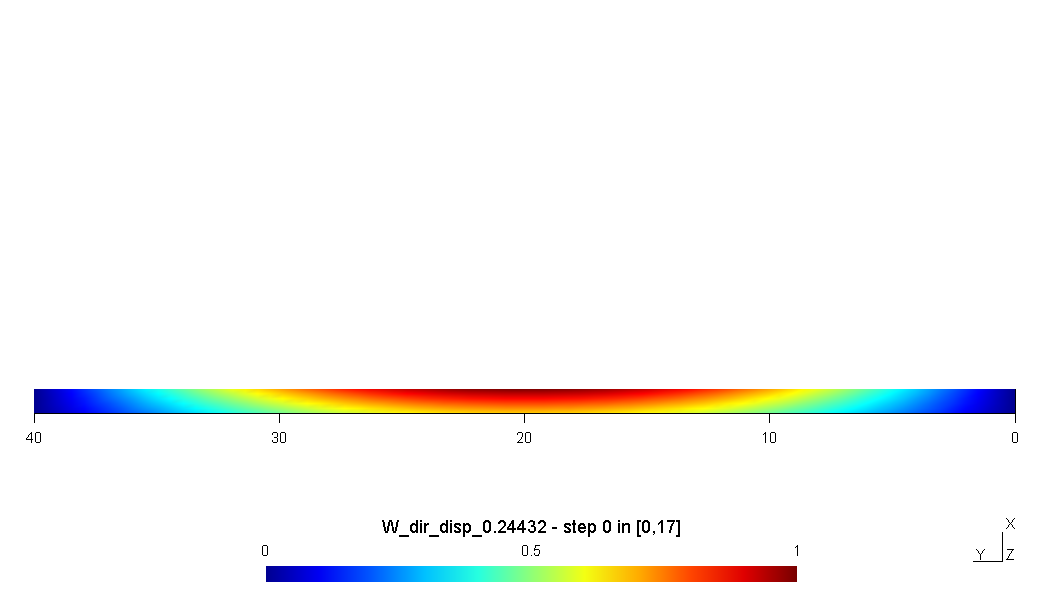
\includegraphics[width=\linewidth,trim={0 3cm 0 9cm},clip]{NAS277/t0_01.png}
\caption{Mode Shape 1 for thickness = 0.01 $(m)$}
\end{subfigure}\vfill
\begin{subfigure}{.8\textwidth}
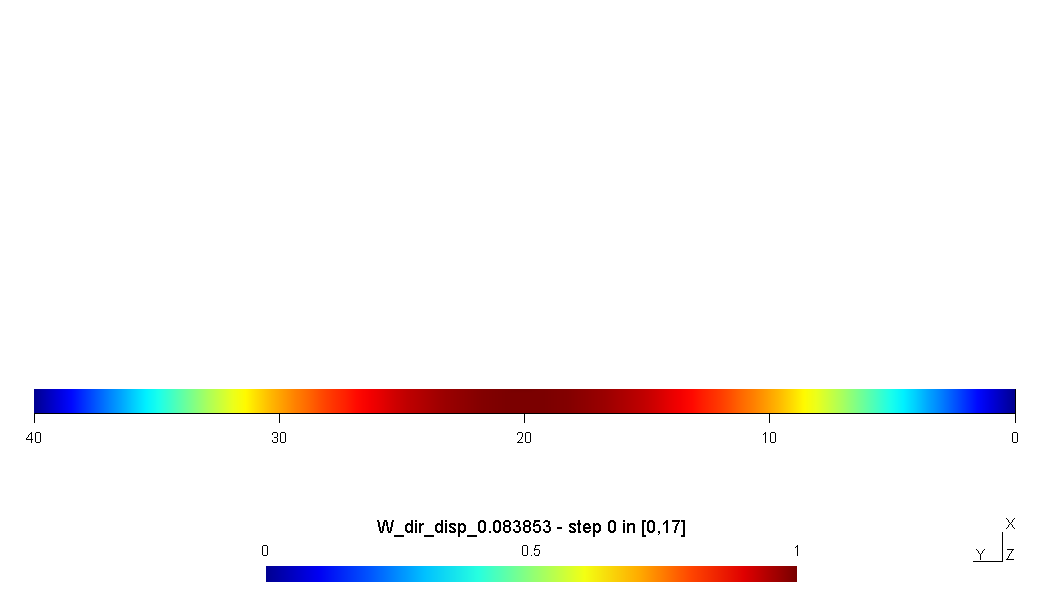
\includegraphics[width=\linewidth,trim={0 3cm 0 9cm},clip]{NAS277/t0_1.png}
\caption{Mode Shape 1 for thickness = 0.1 $(m)$}
\end{subfigure}\vfill
\begin{subfigure}{.8\textwidth}
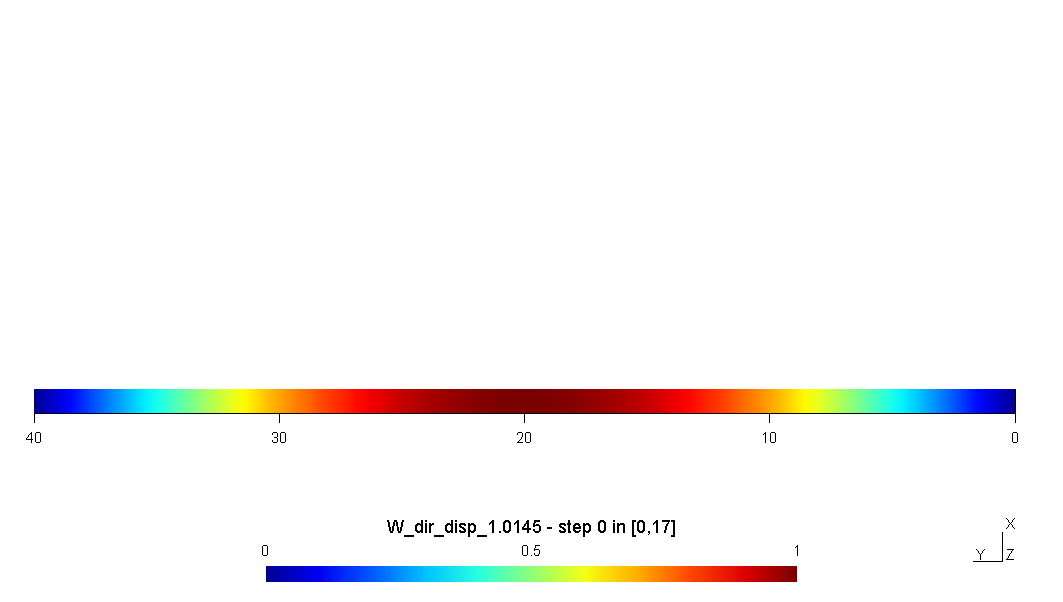
\includegraphics[width=\linewidth,trim={0 3cm 0 9cm},clip]{NAS277/t1.png}
\caption{Mode Shape 1 for thickness = 1 $(m)$}
\end{subfigure} \vfill

\caption{Natural Modes of a rectangular strip}
\end{figure}

\end{document}